\section{MPEG-2 Motion Estimation Subset}


\begin{figure}[t]
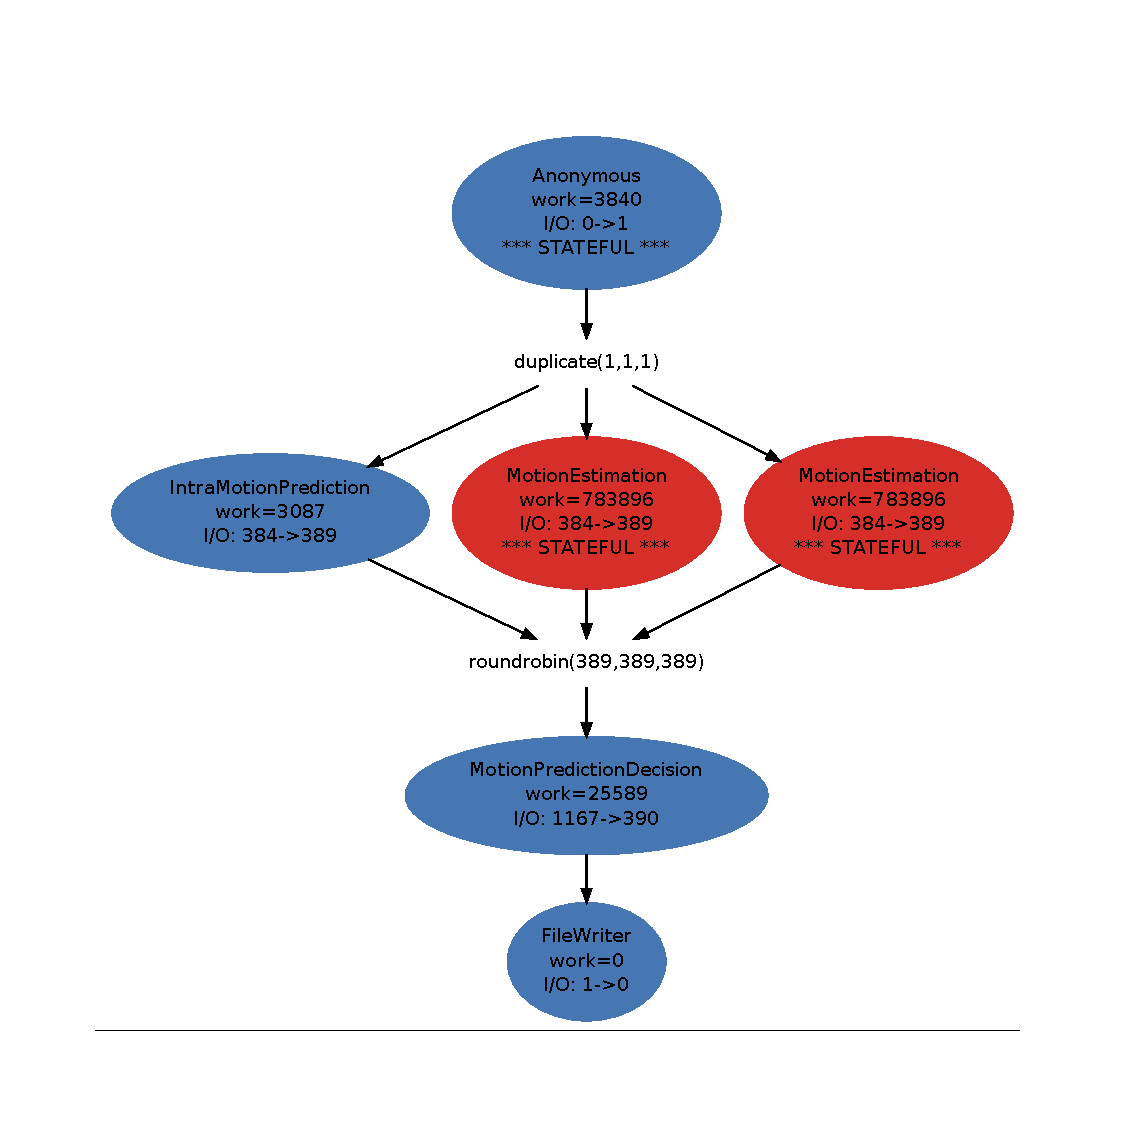
\includegraphics[width=3.5in]{work_estimate_mpeg_motionestimation.pdf}
\caption{MPEG Motion Estimation stream graph.\protect\label{fig:mpegMEgraph}}
\end{figure}


This section presents an application of induction variables to the Motion Estimation compression subset of the MPEG-2 encoder.  MPEG-2 is a standard for coding moving pictures and audio information and has a wide variety of multimedia applications.  

The specification contains various types of compression, one of which is motion prediction.  Motion prediction is a lossless compression, or one that eliminates redundant information from a signal while allowing for an exact reconstruction.  Motion prediction takes advantage of the fact that frames of a video contain a large amount of temporal redundancy.  A particular video sequence often contains duplicated scenes between consecutive frames.  Motion estimation attempts to generate motion predictions with respect to a set of reference frames.  These reference frames can be obtained from previous pictures or from both previous and future pictures.  Accordingly, the MPEG-2 encoder can utilize forward and backward motion estimation to achieve this form of compression.

The MPEG-2 standard organizes pictures into 16x16 groups of pixels called macroblocks.  Each macroblock is itself comprised of four 8x8 blocks of pixels termed as blocks.  Macroblocks can be encoded without any motion prediction, known as intra coded pictures, with only forward motion prediction, known as predictive coded pictures, and with both forward and backward motion prediction, known as bidirectionally predictive coded pictures.  These macroblocks are the basis of MPEG-2 motion prediction.  

The process of Motion Estimation entails comparing macroblocks between frames.  The motion estimator forms a motion vector that indicates a cartesian displacement of the macroblock from the most similar macroblock in the reference frames.  The matching macroblock is also removed from the new macroblock, yielding a residual macroblock that contains the difference between the prediction and the actual macroblock being encoded.  

The Motion estimation stream subgraph of the MPEG-2 encoder is illustrated in Figure~ref{mpegMEgraph}.  Each macroblock will be tested against all three types of prediction (intra coded, forward predicted, and backward predicted) to determine which is the best method for motion estimation.  The MotionEstimationDecision filter determines of these results, which is the best encoding technique.

[cite madrake meng 06]

The work estimation of this compression indicates the filter MotionEstimation is stateful and contains the majority of the work.  The duplicate splitjoin sends a copy of the picture to both forward and backward MotionEstimation and IntraMotionPrediction.  

The MotionEstimation filter pulls macroblocks at a time, iterating through a two-dimensional array (16x16 macroblocks) along the picture.  The filter relies on induction variables to maintain its array position.  We can apply the induction variable transformation on this filter to remove the state in the filter.

Reference pictures are set using upstream messaging from later in the stream graph.  Currently the backend does not support the use of upstream messaging, so for the purpose of benchmarking this application, the reference picture is set to a dummy value and is unchanged throughout the program.  This does not detract from the data parallelism introduced after removing the induction state.  Upstream messaging would simply require that sent messages be duplicated to all fissed filters in the stream graph.

Figure~ref{} shows the runtime figures for the original stateful MPEG-2 motion estimation subset compared to the stateless subset.  We can see significant improvements to runtime after making this subset stateless.  